\section{Durchführung}
\label{sec:Durchführung}
Zur Untersuchung des Photoeffektes wird in diesem Versuch eine Photozelle
verwendet dessen Funktionsweise gleich der in der Theorie \ref{sec:Theorie}
erwähnten Versuchsappertur ist. Die Kathode besteht hier aus einer auf der
Innenseite aufgedampfte Metall- oder Legierungsschicht. Die Anode wird duch einen
Drahtring realisiert der mit minimalem Abstand zur Kathode angebracht wurde.
Die Abbildung \ref{fig:PZ} zeigt eine schemtische Abbildung der Photozelle.
Die Abbildung \ref{fig:VAS} zeigt dagegen den schematischen Versuchsaufbau
der es ermöglicht die Energie der Photoelektronen mit der Gegenfeldmethode zu
bestimmen. Weshalb es möglich ist den vorher erwähnten Zusammenhang \eqref{eqn:Z}
auf
\begin{equation}
  \symup{h} \nu = \symup{e} U_g + A_k
  \label{eqn:hv}
\end{equation}
zu erweitern. Dabei bezeichnet die $\symup{e}$ die Elementarladung und $U_g$ die
Gegenspannung, die multipliziert die kinetischen Energie der Photoelektronen
im Gegenfeld ergeben.
\begin{figure}
  \centering
    \begin{subfigure}{0.48\textwidth}
      \centering
      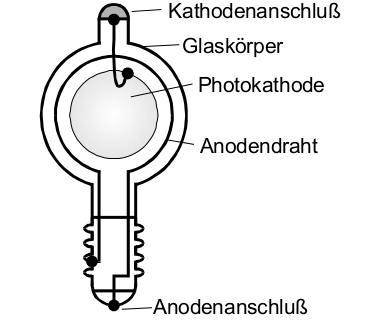
\includegraphics[height=5cm]{logos/Photozelle.png}
      \caption{Die Photozelle - evakuierte Kathode und Anode zur Untersuchung des Photoeffekts \cite{Anleitung}.}
      \label{fig:PZ}
    \end{subfigure}
    \begin{subfigure}{0.48\textwidth}
      \centering
      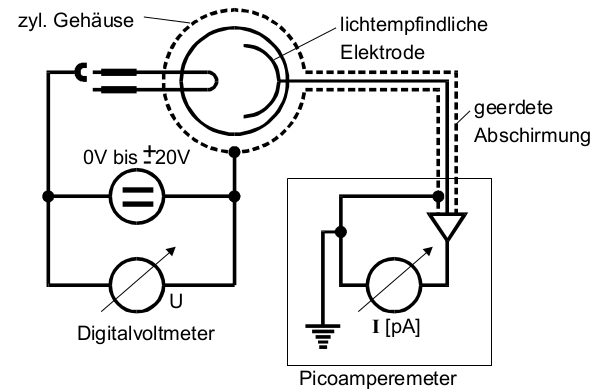
\includegraphics[height=5cm]{logos/VASchaltung.png}
      \caption{Versuchsaufbau zur Messung des Stroms und Bestimmung der Energie der Elektronen durch die Gegenfeldmethode \cite{Anleitung}. }
      \label{fig:VAS}
    \end{subfigure}
  \caption{Schematische Abbildungen}
  \label{fig:PZS}
\end{figure}
Zur Erzeugung monochromatischen Lichtes wird der Versuch wie in Abbildung
\ref{fig:VAO} aufgebaut. Nun müssen erst die Linsen und der Spalt so eingestellt
werden, dass sich das Licht im Prisma bricht und alle Spektrallinien des Lichtes
getrennt, scharf und mit möglichst großer Intensität vor der Photozelle zu beobachten
sind. Dann können die jeweiligen Spektrallinen durch den Schwenkarm auf die
Photozelle gerichtet werden.

\begin{figure}
  \centering
  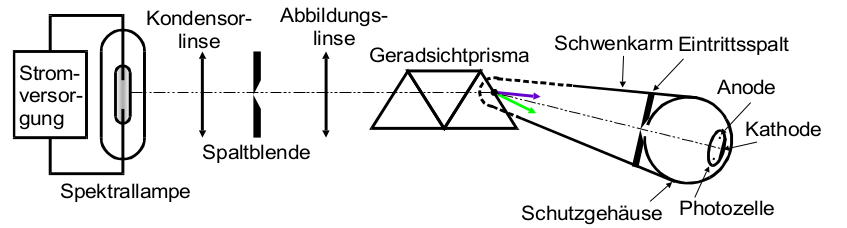
\includegraphics[height=3cm]{logos/VAOptisch.png}
  \caption{Schemtaischer Versuchsaufbau zur Erzeugung des monochromatischen Lichtes \cite{Anleitung}.}
  \label{fig:VAO}
\end{figure}

\paragraph{Messporgramm}
Da hier eine Hg-Dampflampe benutzt wird, wird für alle Spektrallinie der
Photostrom abhängig von der Gegenspannung aufgenommen, außer für die rote Spektrallinie.
Die Spannung wird dabei von $ \SI{-2}{\volt} \leq U \leq \ \SI{2}{\volt}$ variiert.
Dann wird nur für die gelbe Spektrallinie (\SI{578}{\nano\meter}) der Photostrom
abhängig von der Spannung bestimmt. Diesesmal soll aber die Spannung von
\SI{-20}{\volt} bis \SI{20}{\volt} variiert werden.
